\begin{frame}[c]


\begin{center}

\Large{\ALERT{Merck project: \\
Intraocular fluid simulation}}\\

\begin{center}
10th Mathematics Enterprise Study Group\\
Strasbourg
\end{center}

\bigskip
	\footnotesize\textcolor{brunfonce}{June 27th, 2014}
\end{center}

\end{frame}


\section{Problem statement}
\frame{\sectionpage}
\begin{frame}{Eye description}
The eye is the organ of vision; it allows the conversion of light into impulses in neurons.
\begin{center}
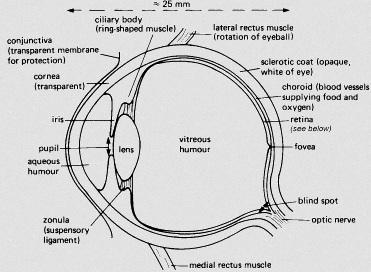
\includegraphics[width=.7\linewidth]{Eye.jpg}
\end{center}
\tiny{source: \url{http://academia.hixie.ch/bath/eye/home.html}}
\end{frame}

\begin{frame}{Eye description}
Aqueous humor: produced by the ciliary epithelium.
$\rightarrow$ drains into the Schlemm's canal.\\
Pressure produced: the intra-ocular pression (IOP).
\begin{center}
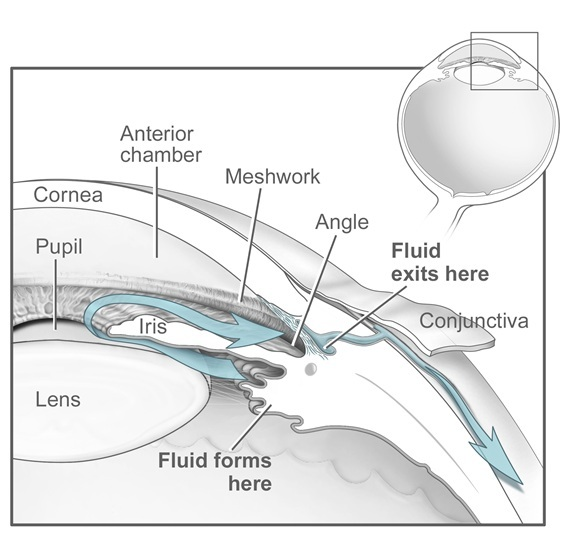
\includegraphics[width=.5\linewidth]{Humor.jpg}
\end{center}


\end{frame}

\begin{frame}{IOP}
IOP : 10 -- 22 mmHg for healthy humans (average : 16 mmHg)
\begin{itemize}
\item inflates the globe of the eye.
\item experimental measure (tonometry) takes into account the thickness of the cornea.
\end{itemize}
%
%
%Note that its value can be measured by tonometry by taking into account the thickness of the cornea. A fine jet of air is directed toward the cornea.
\begin{center}
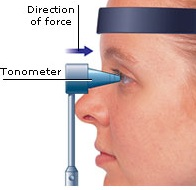
\includegraphics[scale=.6]{Tonometry.jpg}\\
\tiny{source: \url{http://www.aviva.co.uk/health-insurance/home-of-health/medical-centre/medical-encyclopedia/entry/test-tonometry/}}
\end{center}
\only<2>{\begin{center}
\ALERT{High IOP $\Rightarrow$ major risk for \textit{glaucoma}. IT IS ACKWARD TO ALREADY MENTION GLAUCOMA BEFORE INTRODUCING IT (next slide) ...}
\end{center}}
\end{frame}

\begin{frame}{Glaucoma}
%The glaucoma, also called the silent thief of sight, is known as the second leading cause of blindness worldwide (1 in 40 adults over 40 years old).
%\newline
%\\
\begin{itemize}
\item Second leading cause of blindness worldwide (1 in 40 adults over 40 years old)\footnote{\textit{Relative roles of risk factors in the evaluation of a glaucoma suspect : clinical perspective and mthematical modelling},Geffen, Guidoboni, Harris \textit{et al}}
\end{itemize}
% Until now, the major risk for glaucoma is the elevated IOP but it is neither required nor enough to actually contract the disease:\\
Elevated IOP : major risk for glaucoma, but :
\begin{itemize}
\item a patient with an elevated IOP may never contract glaucoma.
\item a patient could have a glaucoma even though his/her IOP is low
\end{itemize}
\begin{center}
\alert{ 25 \% of IOP-treated patient progress to blindness}

\end{center}

\end{frame}

\begin{frame}{Glaucoma}
Group of ocular disorders with multi-factorial etiology united by a clinically characteristic optic neuropathy accompanied by a vision loss.
%\newline
%\\
There are two kinds of diagnostics: \\
\begin{itemize}
\item<2-> a morphological damage
\item<3->a functional damage (decrease of the visual field)
\end{itemize}
\only<2>{
\begin{center}
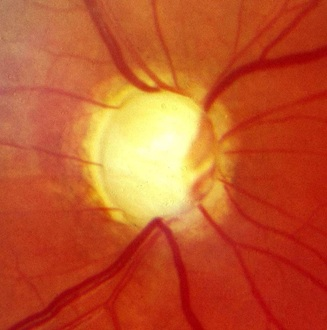
\includegraphics[scale=.5]{Morphological.jpg}\\
\tiny{Glaucomateous optic nervehead demonstrating increased cup to disc ratio}
\end{center}
Glaucoma damages the optical nerve head, where the optical nerve and blood vessels enter the retina.}
\only<3>{

\begin{center}
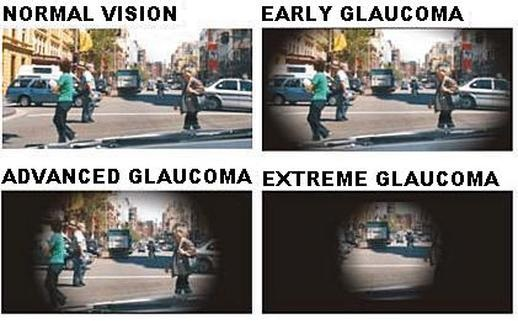
\includegraphics[scale=.5]{Glaucoma.jpg}\\
\tiny{source: \url{http://www.swisscompleteeyecare.com/uploads/3/6/3/8/3638142/8901258.jpg?520}}

\end{center}}
\only<4>{
\begin{center}
\ALERT{
Even though IOP is certainly not the only risk factor in glaucoma, \\ the IOP remains the only parameter we can act on, \\ either by surgery or with medications.
}\end{center}}
\end{frame}

\begin{frame}[shrink=5]{Treatment}

The medications have two effects:
%: either decrease the secretion of aqueous humor or increase the elimination of it. It is also possible to combine several treatments in order to decrease even more the IOP.
\newline
\\
\begin{tabular}{|c|c|}
\hline
Decrease the secretion & Increase the elimination \\
of aqueous humor &  of aqueous humor\\
\hline
beta-adrenergic receptor antagonists & Prostaglandin analogs \\
Alpha2-adrenergic agonists & Miotic agents \\
alpha agonists &  \\
Carbonic anhydrase inhibitors &  \\
\hline
\end{tabular}
\newline
\newline

\textcolor{red}{may be shorten / reformulate the second part of this slide}
It is also possible to combine several treatments in order to decrease even more the IOP.
Besides, drugs could work better on patients depending on their age, gender, ethnic group or other diseases like diabetes, hypertension...

\end{frame}

\begin{frame}

\textcolor{red}{add some transition between clinics and math; what are the open questions?
why the statistical studies are not sufficient to explain what is happening? $\Rightarrow$ math modeling
is needed (you may use ideas from Alon's presentation, slides 19 -- 22).}
\end{frame}
\section{Mathematical Model}
\frame{\sectionpage}
\begin{frame}{Model of intraocular fluids dynamics}
\begin{block}{}
\[
\frac{\dd U}{\dd t}=F_{h}-F_{e}
\]
\end{block}
\begin{itemize}
\item $U$: Total aqueous humor
\item $F_h$: Fluid inflow in posterior chamber
\item $F_e$: net outflow via trabecular path
\end{itemize}

\begin{center}
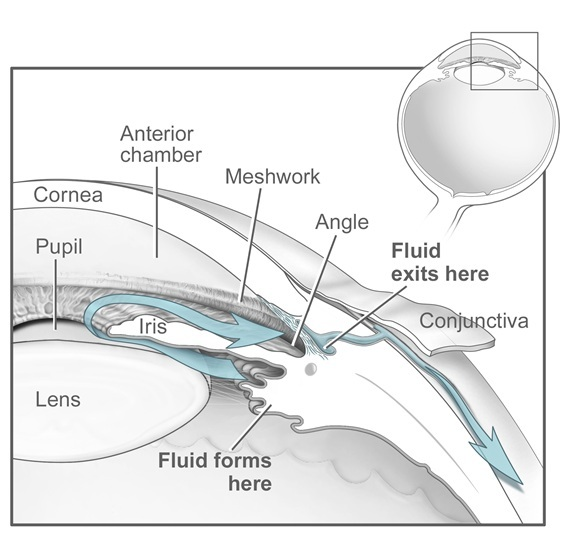
\includegraphics[width=.4\linewidth]{Humor.jpg}
\end{center}

\end{frame}

\begin{frame}{Model of intraocular fluids dynamics}

\[
F_{h}= L_p \big[ (p_a-p)-\sigma_{p} \Delta\pi_{p}-\sigma_{s} \Delta\pi_{s}\big]
\]

\only<1>{
\begin{itemize}
\item $L_p$: permeability of the equivalent membrane
\item $p_a$: pressure in the ciliary body capillaries
\item $p$: IOP
\item $\sigma_p$: reflection coefficient (proteins)
\item $\sigma_s$: reflection coefficient (low molecular components)
\item $\Delta \pi_p $: osmotic pressure diff. accross membrane (proteins)
\item $\Delta \pi_s $: osmotic pressure diff. across membrane (low molecular component)
\end{itemize}}
\only<2>{
\[
\Delta\pi_{s}= \rho(C_1-C_{2})
\]
\begin{itemize}
\item $\rho$: universal gas constant $\times$  absolute temperature
\item $C_1$: total molar concentration of low-molecular components (blood)
\item $C_2$: total molar concentration of low-molecular components (intra-ocular fluid near ciliary body surface)
\item \textcolor{red}{already mention initial conditions?}
\end{itemize}
}
\end{frame}

\begin{frame}{Model of intraocular fluids dynamics}
\[
F_{e}= \frac{p - p_e}{R}
\]
\begin{itemize}

\item $p_e$: pressure in the episcleral veins
\item $R$: output hydraulic resistance
\end{itemize}
\end{frame}



\begin{frame}{Stationary case}
\Alert{Assumption :} inflow rate = outflow rate
\begin{block}{}
\[
F_h = L_p \left(p_a-p-\Delta \pi_p - \sigma_s \Delta\pi_s\right) = \frac{p - p_e}{R}, \; \Delta \pi_s = \rho(C_1-C_2)
\]
\[
F_h (1 - \sigma_s) \overline{C} + J = F_hC_2 , \; \overline{C}= C_1+C2
\]

\end{block}
\begin{figure}[H]
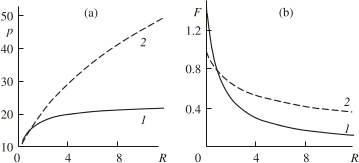
\includegraphics[scale=0.7]{images/courbes_pr_fr}
\end{figure}
%\textcolor{red}{Not clear what are cases 1 and 2}
\begin{center}
\tiny{source : \textit{Dynamic of the intraocular fluid}Lyobimov et al, 2007}
\end{center}
\small{$1$: Purely hydraulic model ($\Delta\pi_s$ is constant)\\
$2$: Osmotic components dynamics ($J$ is constant)}
\end{frame}


\begin{frame}{Nonstationary case}
Linearisation of $V(p)$
\[
V = V(p) \approx V_0 + \alpha (p-p_0)
\]
$\alpha$ : volume compliance of the eye shell (directly measured in experiments/varies significantly)

\begin{block}{}
\[
 \alpha \frac{dp}{dt}=F_{h}-\frac{p-p_e}{R}
 \]
\[
 V^{\ast} \frac{dC_{2}}{dt}= F_h(1-\sigma_s)\overline{C} + J - F_hC_2,\; \overline{C}= \frac{C_1+C_2}{2}
 \]
\end{block}

$V^\star$: volume of intraocular fluid between the folds of the ciliary body\\
$J$: Influx due to active transport

\end{frame}

%\section{Mathematical Model}
%\frame{\sectionpage}
%\begin{frame}{Model of intraocular fluids dynamics}
%\begin{block}{}
%\[
%\frac{\dd U}{\dd t}=F_{h}-F_{e}
%\]
%\end{block}
%\begin{itemize}
%\item $U$: Total aqueous humor
%\item $F_h$: Fluid inflow in posterior chamber
%\item $F_e$: net \textcolor{red}{outflow} via trabecular path \textcolor{red}{formula in the sequel?}
%\end{itemize}
%
%
%
%
%\[
%F_{h}= L_p \big[ (p_a-p)-\sigma_{p} \Delta\pi_{p}-\sigma_{s} \Delta\pi_{s}\big]
%\]
%
%\only<1>{
%\begin{itemize}
%\item $L_p$: permeability of the equivalent membrane
%\item $p_a$: pressure in the ciliary body capillaries
%\item $p$: IOP
%\item $\sigma_p$: reflection coefficient (proteins)
%\item $\sigma_s$: reflection coefficient (low molecular components)
%\item $\Delta \pi_p $: osmotic pressure diff. accross membrane (proteins)
%\item $\Delta \pi_s $: osmotic pressure diff. across membrane (low molecular component)
%\end{itemize}}
%\only<2>{
%\[
%\Delta\pi_{s}= \rho(C_1-C_{2})
%\]
%\begin{itemize}
%\item $\rho$: universal gas constant $\times$  absolute temperature
%\item $C_1$: total molar concentration of low-molecular components (blood)
%\item $C_2$: total molar concentration of low-molecular components (intra-ocular fluid near ciliary body surface)
%\item \textcolor{red}{already mention initial conditions?}
%\end{itemize}
%}
%\end{frame}
%
%\begin{frame}{Stationary case}
%\Alert{Assumption :} inflow rate = outflow rate
%\begin{block}{}
%\[
%F_h = L_p \left(p_a-p-\Delta \Pi_p - \sigma_s \Delta\Pi_s\right) = \frac{p - p_e}{R}, \; \Delta \Pi_s = \rho(C_1-C_2)
%\]
%\[
%F_h (1 - \sigma_s) \overline{C} + J = F_hC_2 , \; \overline{C}= C_1+C2
%\]
%
%\end{block}
%\begin{figure}[H]
%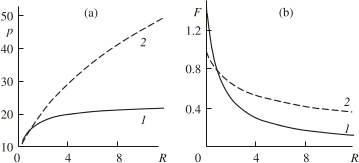
\includegraphics[scale=1]{images/courbes_pr_fr}
%\end{figure}
%\textcolor{red}{Not clear what are cases 1 and 2}
%\tiny{source : \textit{Dynamic of the intraocular fluid}Lyobimov et al, 2007}
%\end{frame}
%
%\begin{frame}{Nonstationary case}
%Linearisation of $V(p)$
%\[
%V = V(p) \approx V_0 + \alpha (p-p_0)
%\]
%$\alpha$ : volume compliance of the eye shell (directly measured in experiments/varies significantly)
%
%\begin{block}{}
%\[
% \alpha \frac{dp}{dt}=F_{h}-\frac{p-p_e}{R}
% \]
%\[
% V^{\ast} \frac{dC_{2}}{dt}= F_h(1-\sigma_s)\overline{C} + J - F_hC_2,\; \overline{C}= \frac{C_1+C_2}{2}
% \]
%\end{block}
%
%$V^\star$: volume of intraocular fluid between the folds of the ciliary body\\
%$J$: Influx due to active transport
%$p_e$: pressure in the episcleral veins\\
%$R$: output hydraulic resistance\\
%
%\end{frame}

%
\section{Numerical Results}
\frame{\sectionpage}
\begin{frame}{Resolution}
\begin{itemize}
\item ODE system : Octave \texttt{ode45} (RK (4,5))
\item Data set from litterature\footnote{Lyubimov et al, 2007,Anders, 1975,The mechanism of aqueous humour formation,2002}
\item Osmotic difference assumed constant
\item Initial values : physiological range
\item Neglecting oscillating component
\end{itemize}

\end{frame}
\begin{frame}
\begin{figure}[h]

\begin{center}
  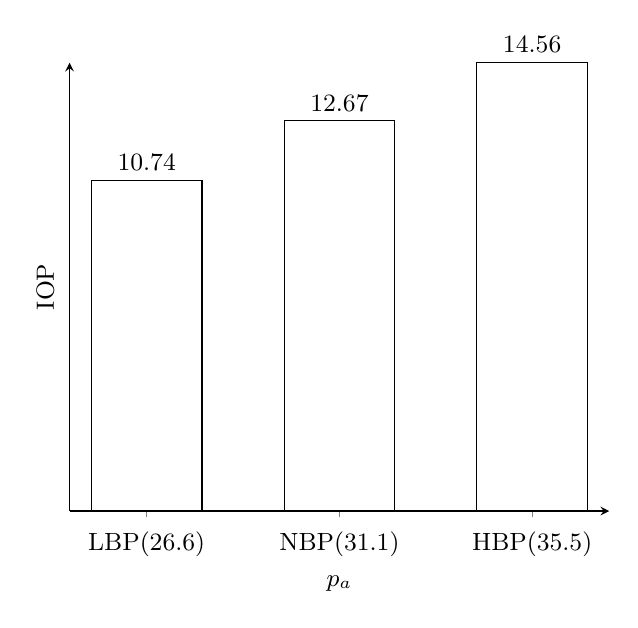
\begin{tikzpicture}[font=\small]
    \begin{axis}[
      ybar,
      bar width=40pt,
      xlabel={$p_a$},
      ylabel={IOP},
      ymin=0,
      ytick=\empty,
      xtick=data,
      axis x line=bottom,
      axis y line=left,
      enlarge x limits=0.2,
      %symbolic x coords={excellent,good,average,bad,awful},
      symbolic x coords = {LBP(26.6),NBP(31.1),HBP(35.5)},
      xticklabel style={anchor=base,yshift=-\baselineskip},
      nodes near coords={\pgfmathprintnumber\pgfplotspointmeta}
    ]
      \addplot[fill=white] coordinates {
        (LBP(26.6),10.743)
        (NBP(31.1),12.671)
        (HBP(35.5),14.557)
      };
    \end{axis}
  \end{tikzpicture}
  \end{center}
  \caption{$IOP = f(p_a)$}
\end{figure}
\end{frame}
\begin{frame}
\alert{For $10$ mmHg increase in SBP or DBP $\rightarrow$ increase in IOP in $0.2$ -- $0.5$ mmHg.}\footnote{Dekoule, Weinner}
\bigskip


\begin{tabular}{|l|l|l|l|}
\hline
BP (SBP/DBP)& LBP($100$/$70$)&NBP($120$/$80$) & HBP ($140$/$90$)\\
$p_a$ (mmHg)& $p_a = 26.6$ & $p_a = 31.1$ & $p_a = 35.5$\\
\hline
IOP & $10.74$ & $12.67$ & $14.56$\\
\hline
\end{tabular}
\bigskip
\begin{itemize}
\item[$\star$] $\Delta$ SBP/DBP $\approx 30$ $\rightarrow \Delta$IOP$\approx 2$ mmHg\\

\item[$\star$]SBP/DBP $\rightarrow$ $p_a$ $\rightarrow$ IOP \underline{slightly}\\

\item[$\hookrightarrow$] Good agreement with clinical studies
\end{itemize}

\end{frame}
\begin{frame}{Time evolution of IOP and $C_2$}
\begin{figure}[H]
\begin{minipage}{0.45\linewidth}
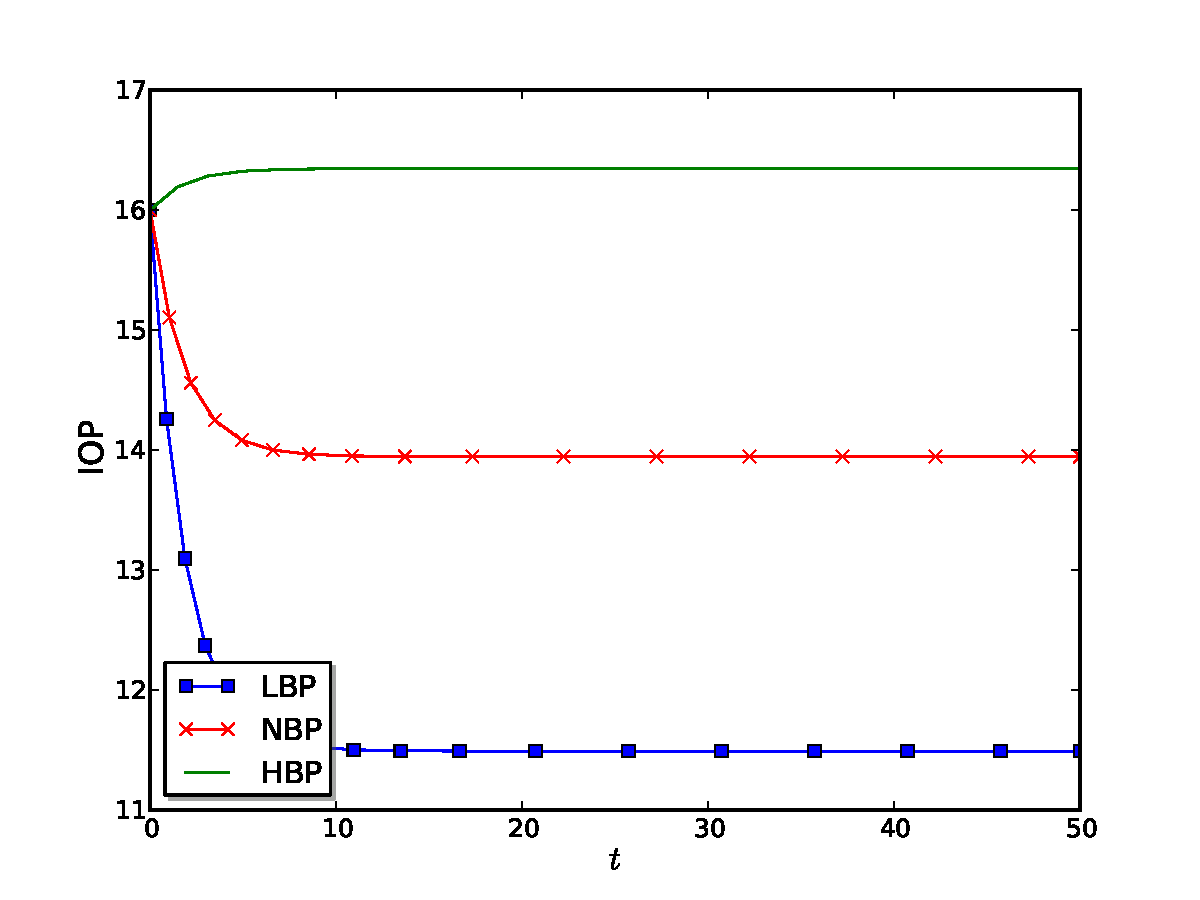
\includegraphics[scale=0.27]{images/IOP_time}
\end{minipage}\hfill
\begin{minipage}{0.45\linewidth}
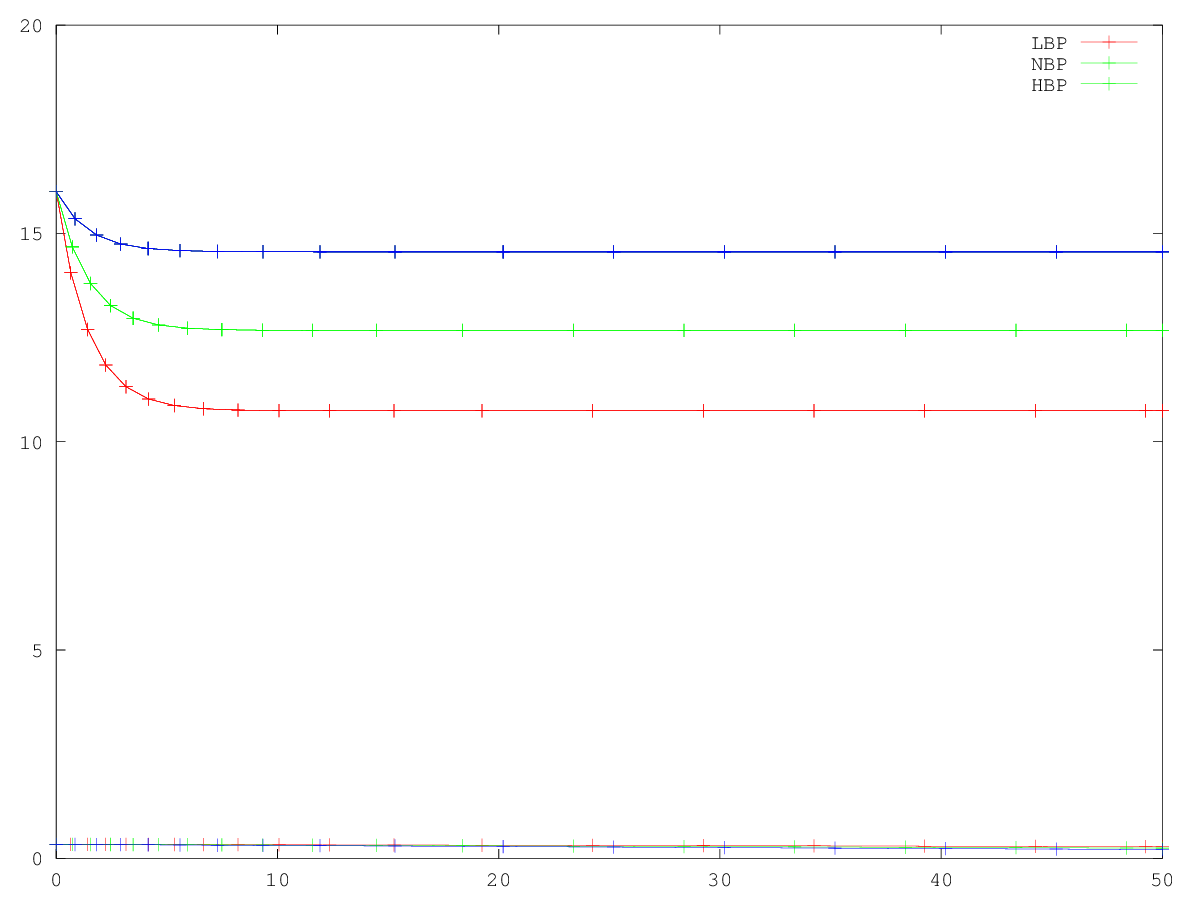
\includegraphics[scale=0.27]{images/C2_time}
\end{minipage}
\end{figure}

\end{frame}

\begin{frame}{The influence of the Outflow resistance R}
\begin{figure}[H]
\begin{minipage}{0.45\linewidth}
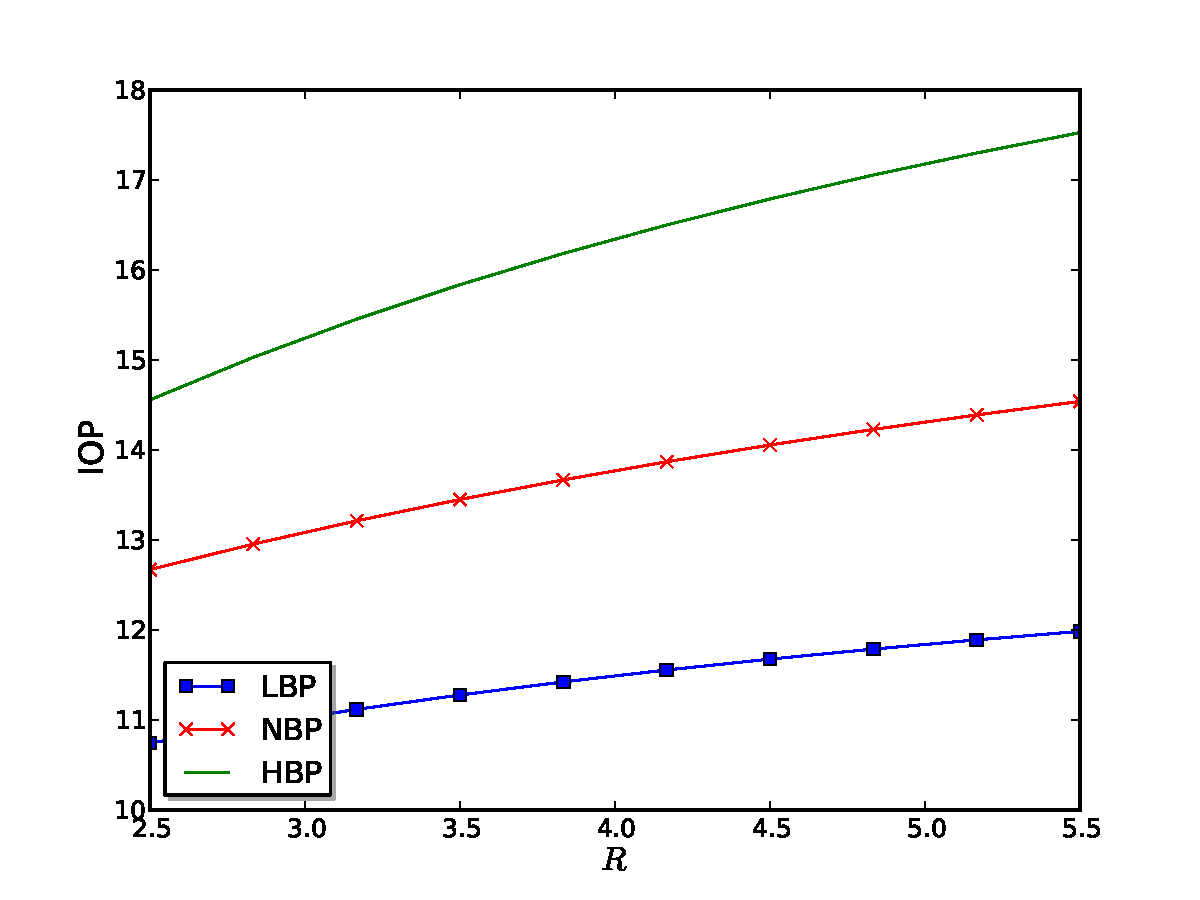
\includegraphics[scale=0.27]{images/IOP_R}
\end{minipage}\hfill
\begin{minipage}{0.45\linewidth}
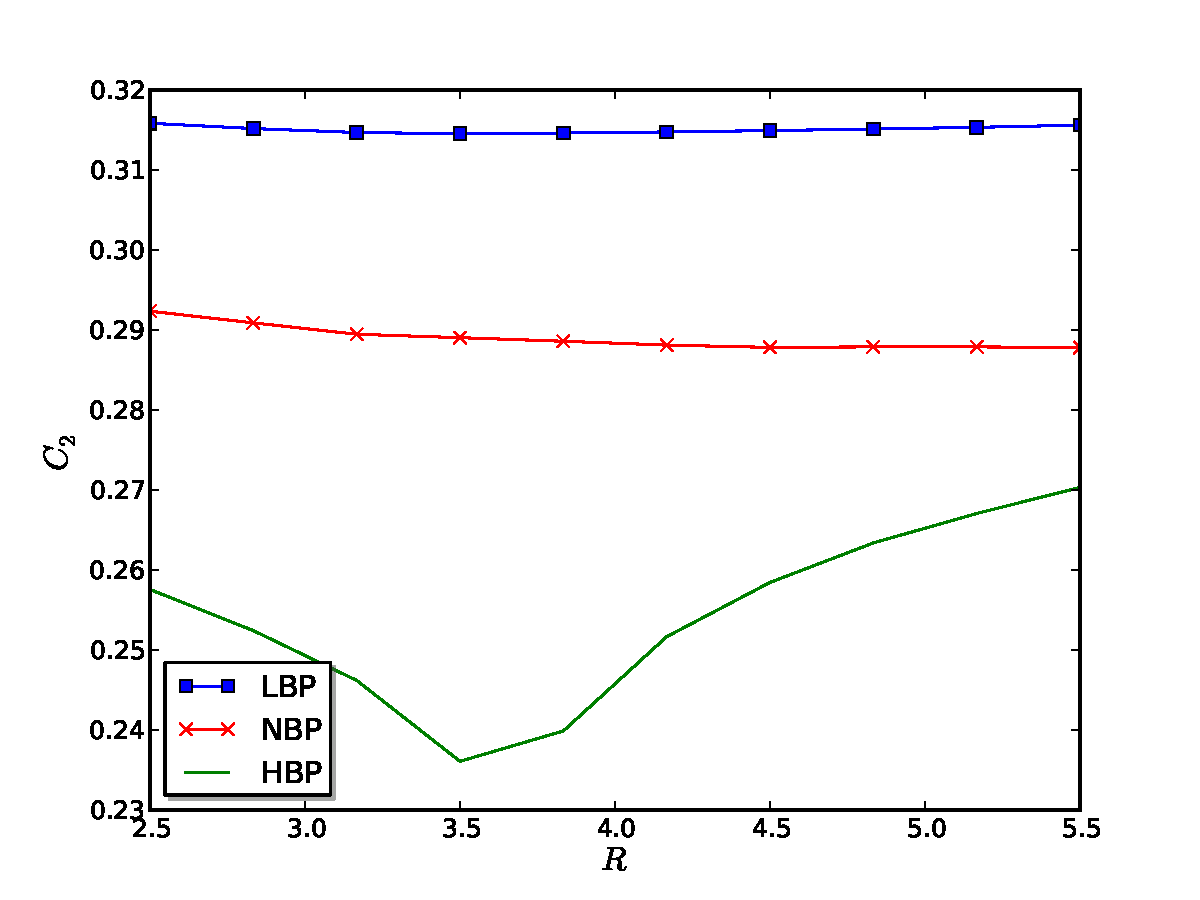
\includegraphics[scale=0.27]{images/C2_R}
\end{minipage}
\end{figure}
\end{frame}
\begin{frame}{The influence of the Outflow resistance R}
\begin{itemize}
\item \alert{HBP }: $\Delta$IOP $\approx 3$ mmHg
$\Rightarrow\frac{\Delta \mathrm{IOP}}{\Delta \mathrm{R}} \approx 1$
\medskip

\item \alert{NBP }: $\Delta$IOP $\approx 2.2$ mmHg
$\Rightarrow
\frac{\Delta \mathrm{IOP}}{\Delta \mathrm{R}} \approx 0.7$
\medskip
\item \alert{LBP }: $\Delta$IOP $\approx 1.1$ mmHg
$\Rightarrow
\frac{\Delta \mathrm{IOP}}{\Delta \mathrm{R}} \approx 0.3$
\end{itemize}
\bigskip
\ALERT{Decreasing inflow resistance : larger IOP reduction for HBP patients}
\end{frame}
\begin{frame}{The influence of inflow permeability $L_p$}
\begin{figure}[H]
\begin{minipage}{0.45\linewidth}
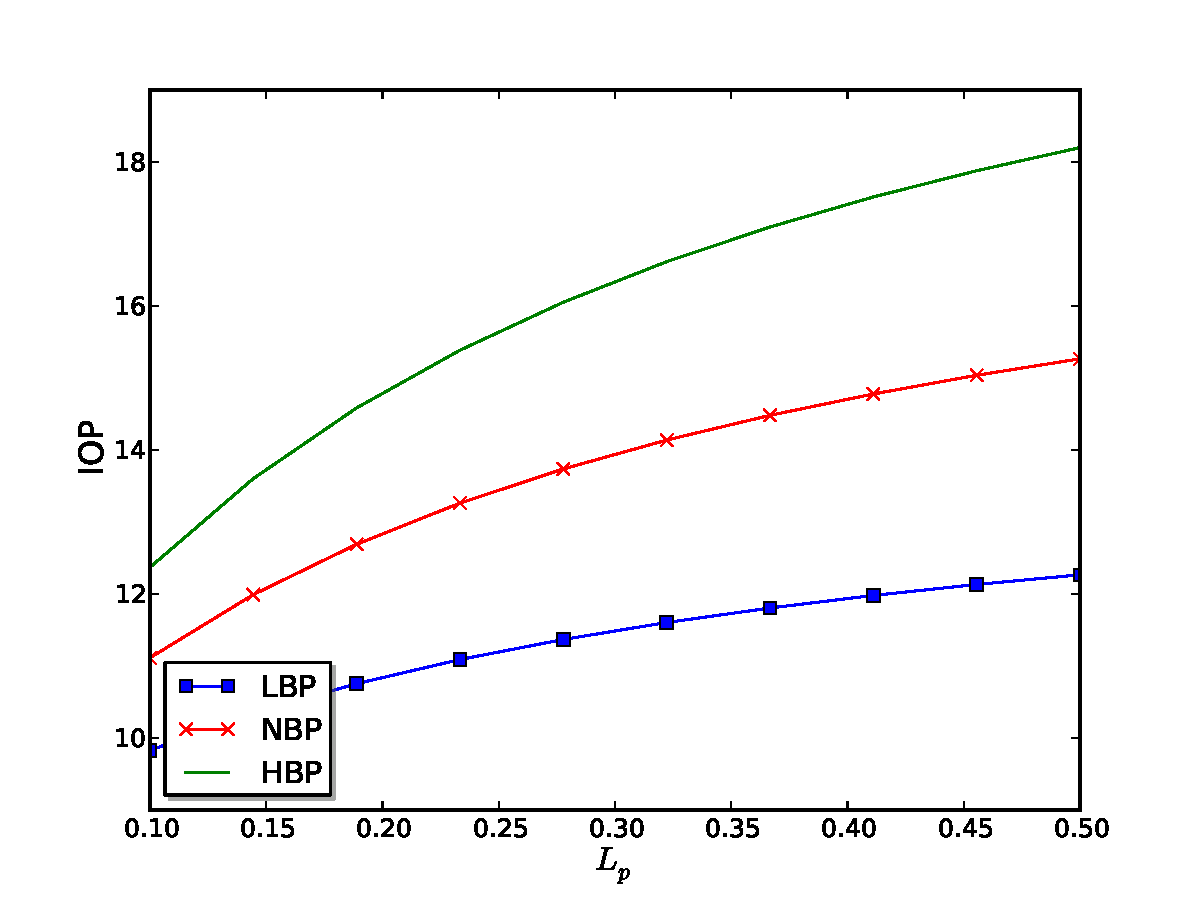
\includegraphics[scale=0.27]{images/IOP_Lp}
\end{minipage}\hfill
\begin{minipage}{0.45\linewidth}
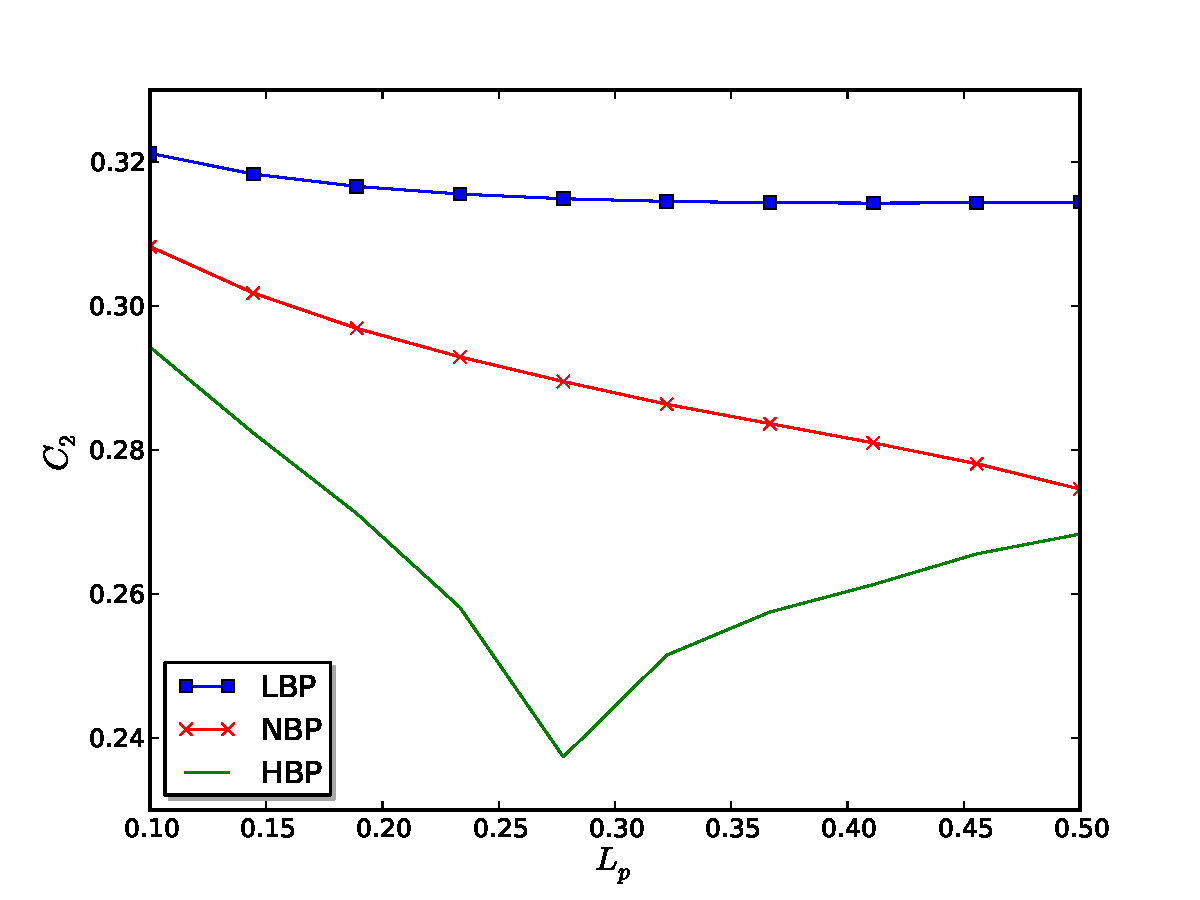
\includegraphics[scale=0.27]{images/C2_Lp}
\end{minipage}
\end{figure}

\end{frame}

\begin{frame}{The influence of inflow permeability $L_p$}
\begin{itemize}
\item \alert{HBP }: $\Delta$IOP $\approx 5.9$ mmHg
$\Rightarrow\frac{\Delta \mathrm{IOP}}{\Delta \mathrm{R}} \approx 15$
\medskip

\item \alert{NBP }: $\Delta$IOP $\approx 4$ mmHg
$\Rightarrow
\frac{\Delta \mathrm{IOP}}{\Delta \mathrm{R}} \approx 10$
\medskip
\item \alert{LBP }: $\Delta$IOP $\approx 3.2$ mmHg
$\Rightarrow
\frac{\Delta \mathrm{IOP}}{\Delta \mathrm{R}} \approx 8$
\end{itemize}
\bigskip
\begin{itemize}
\item[$\star$] Larger IOP reduction for HBP patients
\medskip
\item[$\star$] Decreasing inflow permeability has overalll larger influence on IOP reduction than decreasing outflow resistance
\end{itemize}
\end{frame}

%\begin{frame}{$\sigma_s$ influence}
%\begin{figure}[H]
%\begin{minipage}{0.45\linewidth}
%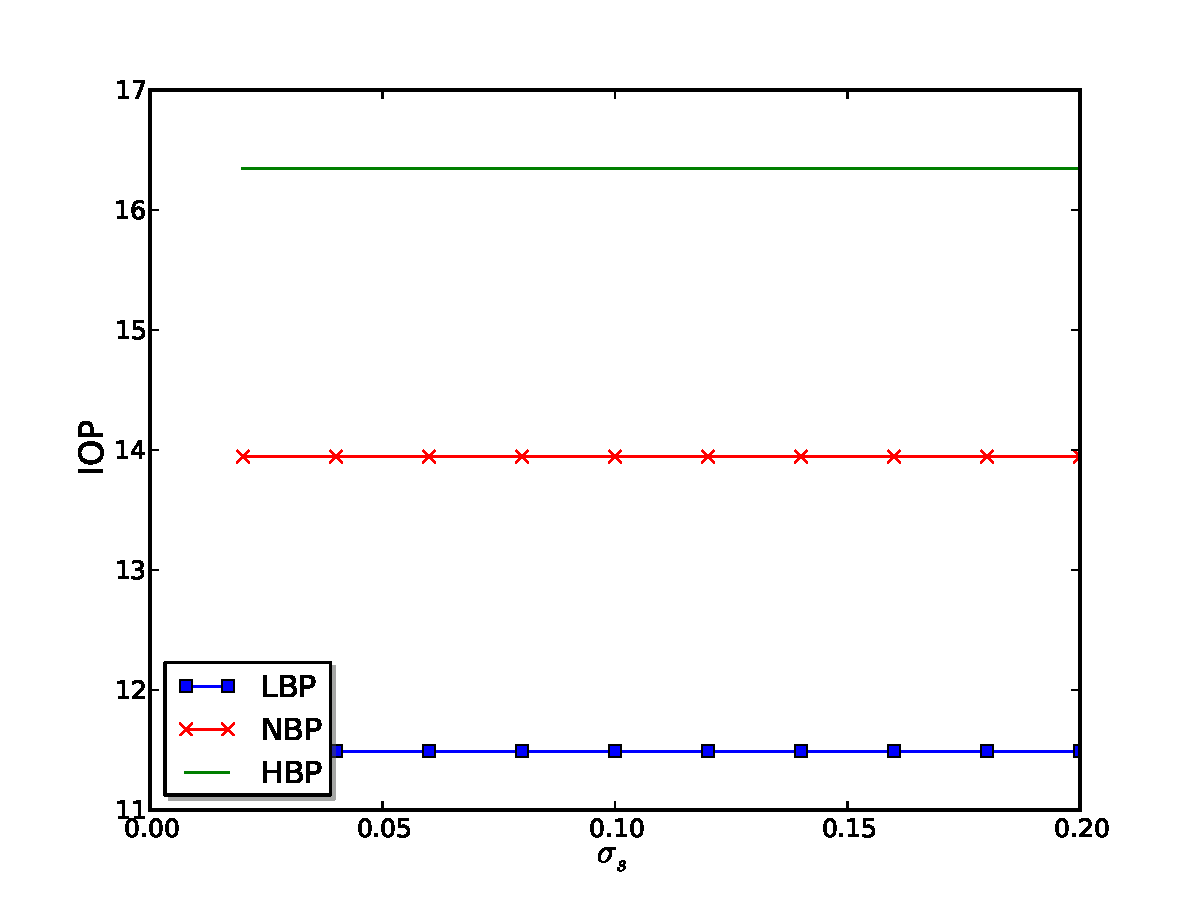
\includegraphics[scale=0.27]{images/IOP_sigmas}
%\end{minipage}\hfill
%\begin{minipage}{0.45\linewidth}
%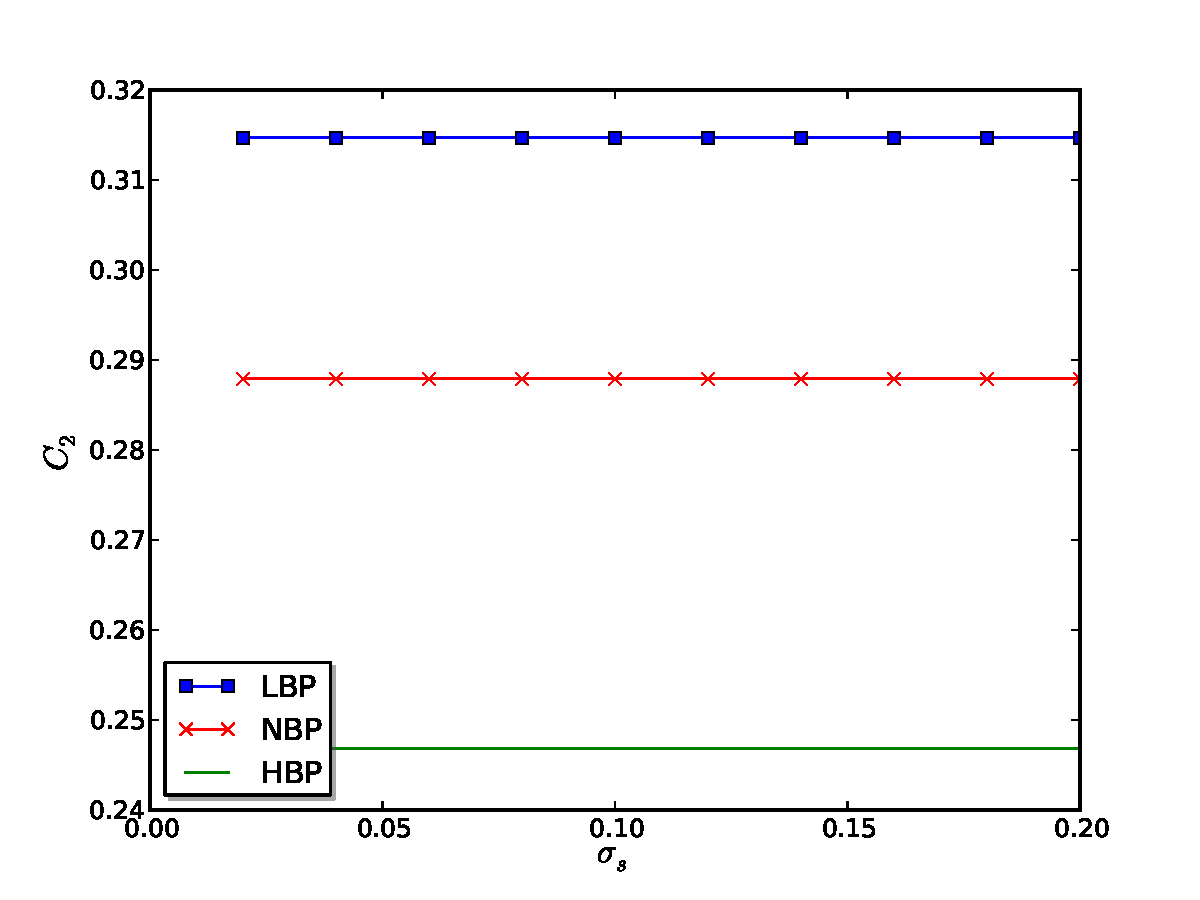
\includegraphics[scale=0.27]{images/C2_sigmas}
%\end{minipage}
%\end{figure}
%
%\end{frame}
\section{Sumary, conclusions and perspectives}
\begin{frame}{Summary}
\begin{itemize}
\item First numerical simulation of relations between blood pression and IOP
\item Model suggests that IOP medication would have different efficacy in individual with different blood pressure
\item Reduction of inflow permeability ($L_p$) gives larger IOP reductions thant reduction of outflow resistance ($R$)
\end{itemize}
\end{frame}
\begin{frame}{Conclusions and perspectives}
\ALERT{Model extensions}
\begin{itemize}
\item Distinguish anterior and posterior chamber
\item Compliance of cornea (anterior chamber)/ sclera (posterior chamber)
\item<2> Comparing model results with clinical studies (stats)
\end{itemize}
\only<1>{\begin{figure}[H]
\begin{center}
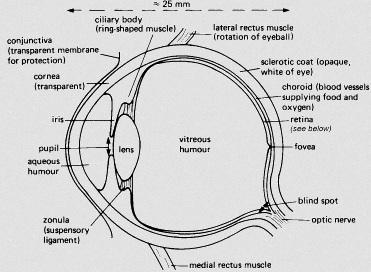
\includegraphics[scale = 0.7]{Eye.jpg}
\end{center}
\end{figure}
\tiny{source: \url{http://academia.hixie.ch/bath/eye/home.html}}
}


\only<2>{\ALERT{Perspectives}
\begin{itemize}
\item Coupling with mathematical model of retinal blood flow
\item Inclusion of oscillations in choroidal blood volume
\item Modeling the relationship between IOP, blood pressure, intracranial pressure
\end{itemize}}
\end{frame}
